% figure: 自控-状态空间结构图.png
% 用途：自控 01-1 状态变量与模拟结构图 —— ẋ=Ax+Bu, y=Cx+Du 的模拟结构图
% 构建：..\build.ps1 -File \block-statespace.tex
% 说明：旧图是通用绘图工具产物：D 支路与 C→求和点 的箭头几乎相接、积分器内的
%       "ẋ→x" 与输入线重叠、D 支路标注 Du 与 C 支路 Cx+Du 挤在一处。
%       本图重新排布垂直间距：D 块上移，C 支路与反馈支路分层走线。
\documentclass[border=10pt]{standalone}
\usepackage{fontspec}
\setmainfont{Cambria}
\usepackage{unicode-math}
\setmathfont{Cambria Math}
\usepackage{tikz}
\usetikzlibrary{positioning, arrows.meta, calc, decorations.pathmorphing}
\usepackage{ctex}

\definecolor{figink}{HTML}{1E2228}
\definecolor{figacc}{HTML}{B23020}
\definecolor{figsub}{HTML}{606874}
\definecolor{figfill}{HTML}{E8EFF8}

\begin{document}
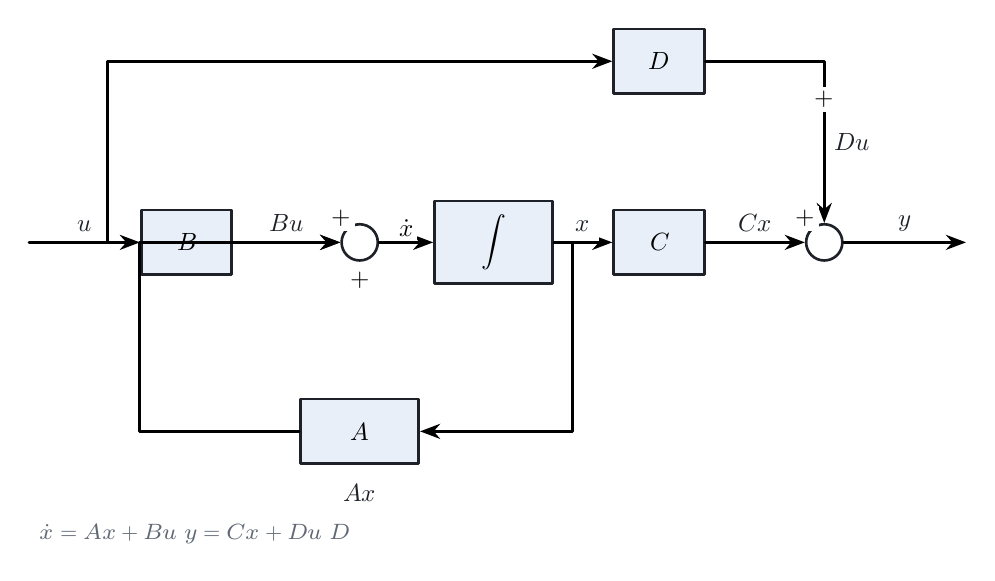
\begin{tikzpicture}[
  x=1cm, y=1cm,
  line width=0.95pt, line cap=round, line join=round,
  >=Stealth,
  blk/.style = {draw=figink, line width=0.95pt, fill=figfill,
                minimum width=1.15cm, minimum height=0.82cm, inner sep=2pt,
                anchor=center, font=\small},
  int/.style = {draw=figink, line width=0.95pt, fill=figfill,
                minimum width=1.5cm, minimum height=1.05cm, inner sep=2pt,
                anchor=center, font=\small},
  sum/.style = {draw=figink, line width=0.95pt, circle, inner sep=0pt,
                minimum size=0.46cm, anchor=center},
  sig/.style = {font=\small, color=figink, fill=white},
  sub/.style = {font=\footnotesize, color=figsub, fill=white},
  lbl/.style = {font=\small, inner sep=1.5pt, fill=white}
]

% 主通道 y=0
\node[blk] (b)  at (0,0)    {$B$};
\node[sum] (s1) at (2.2,0)  {};
\node[int] (i)  at (3.9,0)  {$\displaystyle\int$};
\node[blk] (c)  at (6.0,0)  {$C$};
\node[sum] (s2) at (8.1,0)  {};

% 上方 D 支路 y=2.3
\node[blk] (d) at (6.0,2.3) {$D$};

% 下方 A 反馈支路：放在求和点正下方，反馈线从方框左右两侧引出，不穿框
\node[blk, minimum width=1.5cm] (a) at (2.2,-2.4) {$A$};

% 输入
\draw[->] (-2.0,0) -- node[sig, above] {$u$} (b.west);

% B -> 求和点
\draw[->] (b.east) -- node[sig, above] {$Bu$} (s1.west);

% 求和点 -> 积分器 -> C -> 求和点 -> 输出
\draw[->] (s1.east) -- node[lbl, above] {$\dot x$} (i.west);
\draw[->] (i.east) -- node[sig, above] {$x$} (c.west);
\draw[->] (c.east) -- node[sig, above] {$Cx$} (s2.west);
\draw[->] (s2.east) -- node[sig, above] {$y$} (9.9,0);

% D 支路：u 分支 -> D -> 输出求和点
\draw[->] (-1.0,0) -- (-1.0,2.3) -- (d.west);
\draw[->] (d.east) -- (8.1,2.3) -- node[sig, right] {$Du$} (s2.north);

% A 反馈：x 分支 -> 横线 -> A 方框右侧；方框左侧 -> 绕行 -> 求和点
\draw[->] (4.9,0) -- (4.9,-2.4) -- (a.east);
\draw[->] (a.west) -- (-0.6,-2.4) -- (-0.6,0) -- (s1.west);
\node[sig, below=3pt of a] {$Ax$};

% 求和点符号
\node[lbl] at (1.96,0.30) {$+$};
\node[lbl] at (2.2,-0.48) {$+$};
\node[lbl] at (7.86,0.30) {$+$};
\node[lbl] at (8.1,2.30-0.48) {$+$};

% 结构方程
\node[sub, anchor=west] at (-2.0,-3.7)
  {$\dot x=Ax+Bu$，$y=Cx+Du$（$D$ 支路为直接传递，常为零矩阵）};

\end{tikzpicture}
\end{document}
